\documentclass[tikz]{standalone}

\usepackage{tikz}
\usetikzlibrary{trees}
\usetikzlibrary{shapes}
\usetikzlibrary{positioning}
\usetikzlibrary{arrows.meta}

\tikzset{
    pointer/.style = {thick,draw=black,triangle 45-*,shorten >=-3pt},
    cell/.style = {rectangle, thick, draw=black,minimum width = 1cm, minimum height =1.0cm,fill=yellow!20},
    mynode/.style = {circle, thick, draw=black, align=center,fill=yellow!40,font=\ttfamily\bfseries\Large},
    mynoder/.style = {circle, thick, draw=black, align=center,fill=red!30,font=\ttfamily\bfseries\Large},
    mynodeb/.style = {circle, thick, draw=black, align=center,fill=blue!30,font=\ttfamily\bfseries\Large},
    edgen/.style = {-latex,ultra thick},
    edger/.style = {-latex,ultra thick,red},
    edgeb/.style = {-latex,ultra thick,blue},
    edgeg/.style = {-latex,ultra thick,gray},
    edgegd/.style = {-latex,ultra thick,brown,dashed}, % back
    edgevd/.style = {-latex,ultra thick,violet,dotted}, % forward
    edgexd/.style = {-latex,ultra thick,blue,densely dotted}, % traversal
    every picture/.style={/utils/exec={\ttfamily\bfseries}},
    every picture/.style={font issue=\ttfamily\bfseries},
    font issue/.style={execute at begin picture={#1\selectfont}
  }
}

\newcommand{\R}[1]{\textcolor{red}{#1}}
\newcommand{\B}[1]{\textcolor{violet}{#1}}

\begin{document}

%% 1
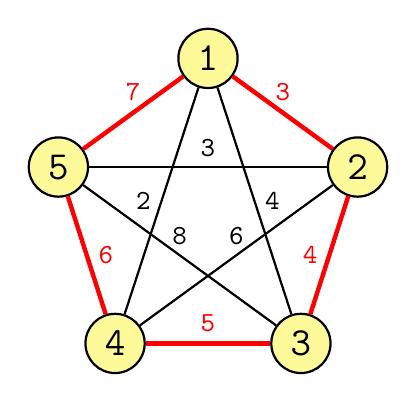
\begin{tikzpicture}[scale=1.00,transform shape]
\node[mynode] at ( 0.00,  3.00) (1) {1};
\node[mynode] at ( 1.90,  1.62) (2) {2};
\node[mynode] at ( 1.18, -0.62) (3) {3};
\node[mynode] at (-1.18, -0.62) (4) {4};
\node[mynode] at (-1.90,  1.62) (5) {5};

\draw[edger, ultra thick,-] (1) edge[above] node {3} (2);
\draw[edgen, thick,-] (1) edge[right] node {4} (3);
\draw[edgen, thick,-] (1) edge[left] node {2} (4);
\draw[edger, ultra thick,-] (1) edge[above] node {7} (5);
\draw[edger, ultra thick,-] (2) edge[left] node {4} (3);
\draw[edgen, thick,-] (2) edge[above] node {6} (4);
\draw[edgen, thick,-] (2) edge[above] node {3} (5);
\draw[edger, ultra thick,-] (3) edge[above] node {5} (4);
\draw[edgen, thick,-] (3) edge[above] node {8} (5);
\draw[edger, ultra thick,-] (4) edge[right] node {6} (5);

\end{tikzpicture}

%% 2
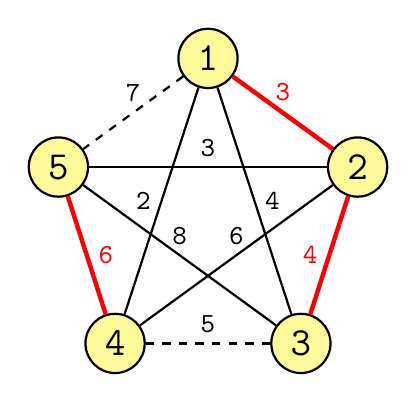
\begin{tikzpicture}[scale=1.00,transform shape]
\node[mynode] at ( 0.00,  3.00) (1) {1};
\node[mynode] at ( 1.90,  1.62) (2) {2};
\node[mynode] at ( 1.18, -0.62) (3) {3};
\node[mynode] at (-1.18, -0.62) (4) {4};
\node[mynode] at (-1.90,  1.62) (5) {5};

\draw[edger, ultra thick,-] (1) edge[above] node {3} (2);
\draw[edgen, thick,-] (1) edge[right] node {4} (3);
\draw[edgen, thick,-] (1) edge[left] node {2} (4);
\draw[edgen, dashed, thick,-] (1) edge[above] node {7} (5);
\draw[edger, ultra thick,-] (2) edge[left] node {4} (3);
\draw[edgen, thick,-] (2) edge[above] node {6} (4);
\draw[edgen, thick,-] (2) edge[above] node {3} (5);
\draw[edgen, dashed, thick,-] (3) edge[above] node {5} (4);
\draw[edgen, thick,-] (3) edge[above] node {8} (5);
\draw[edger, ultra thick,-] (4) edge[right] node {6} (5);

\end{tikzpicture}

%% 3
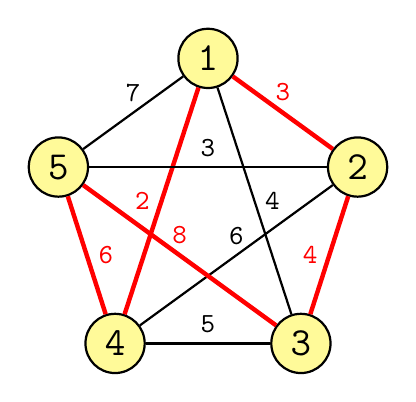
\begin{tikzpicture}[scale=1.00,transform shape]
\node[mynode] at ( 0.00,  3.00) (1) {1};
\node[mynode] at ( 1.90,  1.62) (2) {2};
\node[mynode] at ( 1.18, -0.62) (3) {3};
\node[mynode] at (-1.18, -0.62) (4) {4};
\node[mynode] at (-1.90,  1.62) (5) {5};

\draw[edger, ultra thick,-] (1) edge[above] node {3} (2);
\draw[edgen, thick,-] (1) edge[right] node {4} (3);
\draw[edger, ultra thick,-] (1) edge[left] node {2} (4);
\draw[edgen, thick,-] (1) edge[above] node {7} (5);
\draw[edger, ultra thick,-] (2) edge[left] node {4} (3);
\draw[edgen, thick,-] (2) edge[above] node {6} (4);
\draw[edgen, thick,-] (2) edge[above] node {3} (5);
\draw[edgen, thick,-] (3) edge[above] node {5} (4);
\draw[edger, ultra thick,-] (3) edge[above] node {8} (5);
\draw[edger, ultra thick,-] (4) edge[right] node {6} (5);

\end{tikzpicture}

%% 4
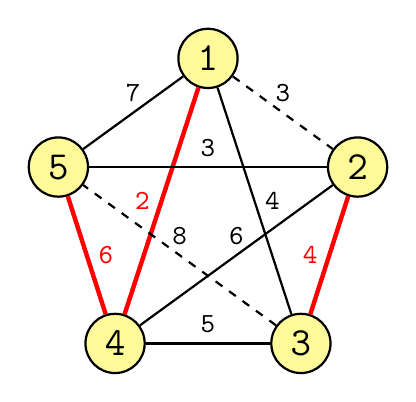
\begin{tikzpicture}[scale=1.00,transform shape]
\node[mynode] at ( 0.00,  3.00) (1) {1};
\node[mynode] at ( 1.90,  1.62) (2) {2};
\node[mynode] at ( 1.18, -0.62) (3) {3};
\node[mynode] at (-1.18, -0.62) (4) {4};
\node[mynode] at (-1.90,  1.62) (5) {5};

\draw[edgen, dashed, thick,-] (1) edge[above] node {3} (2);
\draw[edgen, thick,-] (1) edge[right] node {4} (3);
\draw[edger, ultra thick,-] (1) edge[left] node {2} (4);
\draw[edgen, thick,-] (1) edge[above] node {7} (5);
\draw[edger, ultra thick,-] (2) edge[left] node {4} (3);
\draw[edgen, thick,-] (2) edge[above] node {6} (4);
\draw[edgen, thick,-] (2) edge[above] node {3} (5);
\draw[edgen, thick,-] (3) edge[above] node {5} (4);
\draw[edgen, dashed, thick,-] (3) edge[above] node {8} (5);
\draw[edger, ultra thick,-] (4) edge[right] node {6} (5);

\end{tikzpicture}

%% 5
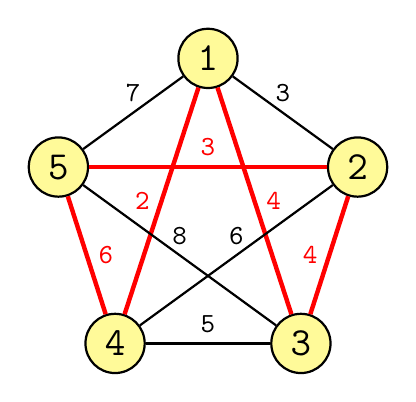
\begin{tikzpicture}[scale=1.00,transform shape]
\node[mynode] at ( 0.00,  3.00) (1) {1};
\node[mynode] at ( 1.90,  1.62) (2) {2};
\node[mynode] at ( 1.18, -0.62) (3) {3};
\node[mynode] at (-1.18, -0.62) (4) {4};
\node[mynode] at (-1.90,  1.62) (5) {5};

\draw[edgen, thick,-] (1) edge[above] node {3} (2);
\draw[edger, ultra thick,-] (1) edge[right] node {4} (3);
\draw[edger, ultra thick,-] (1) edge[left] node {2} (4);
\draw[edgen, thick,-] (1) edge[above] node {7} (5);
\draw[edger, ultra thick,-] (2) edge[left] node {4} (3);
\draw[edgen, thick,-] (2) edge[above] node {6} (4);
\draw[edger, ultra thick,-] (2) edge[above] node {3} (5);
\draw[edgen, thick,-] (3) edge[above] node {5} (4);
\draw[edgen, thick,-] (3) edge[above] node {8} (5);
\draw[edger, ultra thick,-] (4) edge[right] node {6} (5);

\end{tikzpicture}



\end{document}